\subsubsection{Controllable Neural Symbolic Regression}

\citet{bendinelli2023controllable} introduce Neural Symbolic Regression with
Hypotheses (NSRwH). The method receives both a numerical dataset and a set of
user-supplied hypotheses about the desired equation, then generates candidate
expressions conditioned on both sources. It extends the pretrained neural
symbolic-regression pipeline of NeSymReS \citep{biggio2021neural}: synthetic
expressions are sampled and evaluated to create training pairs, while a
Transformer learns the inverse mapping from the evaluated points back to a
prefix expression. NSRwH adds explicit structural control to this inverse
mapping.

\paragraph{How the synthetic expressions and numerical data are sampled.}
Every training example is a triple $(e,\mathcal D,\mathcal H)$. The first two
elements are constructed as follows \citep{bendinelli2023controllable}.

\begin{enumerate}
    \item Sample a random unary--binary expression-tree shape using the
    procedure of Lample and Charton. The paper restricts depth to
    $1,\ldots,6$, prefix length to at most 20 tokens, and the number of input
    variables to at most five. The released configuration also sets a maximum
    of six operator insertions.

    \item Assign an operator of matching arity to every internal node. The
    reported unary library is
    \[
      \{\sqrt{\cdot},(\cdot)^2,(\cdot)^3,(\cdot)^4,
        (\cdot)^{-1},\log,\exp,\sin,\cos,\arcsin\};
    \]
    the binary library is $\{+,-,\times,\div\}$. Leaves receive variables
    $x_1,\ldots,x_5$ or constant placeholders.

    \item Simplify the expression with SymPy. Sample additive constants
    uniformly on $[-10,10]$ and positive multiplicative constants
    log-uniformly on $[0.05,10]$.

    \item For each active variable, sample the two limits of its support from
    $[-10,10]$, requiring an interval width of at least one. Then sample
    $n\in\{1,\ldots,1000\}$ input points independently within those limits.

    \item Evaluate $e$ at the sampled points to obtain
    $\mathcal D=\{(\mathbf x_i,e(\mathbf x_i))\}_{i=1}^{n}$. Inputs producing
    NaNs or magnitudes above the half-precision limit 65504 are discarded and
    resampled.
\end{enumerate}

The official generator makes the first step more precise. It precomputes the
number of unary--binary trees that can complete each combination of open leaf
positions and remaining operators. At each iteration it uses these counts to
sample (i) which still-empty position receives the next operator and (ii)
whether that operator is unary or binary. It then samples the concrete operator
from configurable weights, opens the required child positions, and eventually
fills all remaining positions with variables. This produces a complete prefix
tree with a controlled operator budget rather than growing branches until an
uncontrolled stopping event.\footnote{Official NSRwH implementation:
\href{https://github.com/SymposiumOrganization/ControllableNeuralSymbolicRegression}
{official NSRwH repository}; see \texttt{dataset/generator.py} and
\texttt{configs/dataset\_configuration.json}.}

\paragraph{How the hypotheses are generated.}
During pretraining, $\mathcal H$ is extracted from the known sampled expression
$e$. At inference, the same fields can be supplied by a scientist as complete,
partial, or uncertain prior knowledge.

\begin{table}[tbp]
\centering
\small
\renewcommand{\arraystretch}{1.08}
\begin{tabular}{@{}p{0.22\textwidth}p{0.70\textwidth}@{}}
\toprule
Hypothesis & Information encoded for the expression decoder \\
\midrule
Complexity & Number of operators, variables, and constants in the expression. \\
Symmetry & Tokens indicating whether selected groups of input variables have
generalized symmetry. \\
Positive branches & Prefix subtrees known to occur in $e$. The complete tree
and trivial one-variable branches are excluded. \\
Negative branches & Prefix subtrees selected from the training distribution
and known to be absent from $e$. \\
Known constants & Numerical constant values paired with pointer tokens that
identify where the decoder may place them. \\
\bottomrule
\end{tabular}
\caption{The five hypothesis families used to condition NSRwH.}
\label{tab:nsrwh-hypotheses}
\end{table}

Positive and negative candidate subtrees are enumerated with depth-first
search. A subtree of prefix length $L_s$ is sampled with weight proportional
to $L_s^{-2}$, so short fragments are presented more often. Parameters
$p_{+}$ and $p_{-}$ control the total number of positive and negative tokens:
sampling continues until their aggregate lengths reach approximately
$p_{+}|e|$ and $p_{-}|e|$, respectively. Masking different hypothesis families
during training teaches one model to operate with many levels of available
prior information.

\paragraph{Architecture and controlled expression decoding.}
NSRwH contains a numerical set encoder, a symbolic hypothesis encoder, and an
autoregressive Transformer decoder. Numerical values first receive a 16-bit
multi-hot representation and an embedding. A set Transformer maps the
unordered input--output points to $\mathbf z_{\mathrm{num}}$. A second set
Transformer maps the hypothesis tokens to $\mathbf z_{\mathrm{hyp}}$. Both
outputs have compatible shape and are combined elementwise:

\begin{equation}
\begin{aligned}
\mathbf z_{\mathrm{num}}&=\operatorname{Enc}_{\mathrm{num}}(\mathcal D),\\
\mathbf z_{\mathrm{hyp}}&=\operatorname{Enc}_{\mathrm{hyp}}(\mathcal H),\\
\mathbf z_{\mathrm{fuse}}&=
    \mathbf z_{\mathrm{num}}+\mathbf z_{\mathrm{hyp}},\\
p_{\phi}(e\mid\mathcal D,\mathcal H)
    &=\operatorname{Dec}_{\phi}(\mathbf z_{\mathrm{fuse}}).
\end{aligned}
\label{eq:nsrwh-fusion}
\end{equation}

The decoder predicts the prefix expression token by token and uses beam search
to retain several candidates. Equation~\eqref{eq:nsrwh-fusion} is the source of
controllability: changing $\mathcal H$ changes the decoder distribution without
retraining the network. Known numerical constants use pointer tokens, avoiding
one vocabulary entry for every possible real number. Remaining constants are
fitted with BFGS, after which candidates are ranked by their numerical fit.

The reported model was trained on 200 million expressions using three NVIDIA
RTX 3090 GPUs for five days with batch size 400. The numerical encoder and
expression decoder each use five layers; the hidden dimension is 512. Training
uses teacher-forced next-token cross-entropy, while inference uses beam search.
The paper separates three evaluation questions: \emph{is satisfied} measures
how often decoded expressions obey the supplied hypothesis; \emph{is correct}
requires numerical agreement at more than 99\% of held-out support points; and
mean $R^2$ measures numerical fit. This distinction prevents an expression that
obeys the requested structure but predicts poorly from being counted as a
successful mechanism recovery.

\begin{figure}[H]
\centering
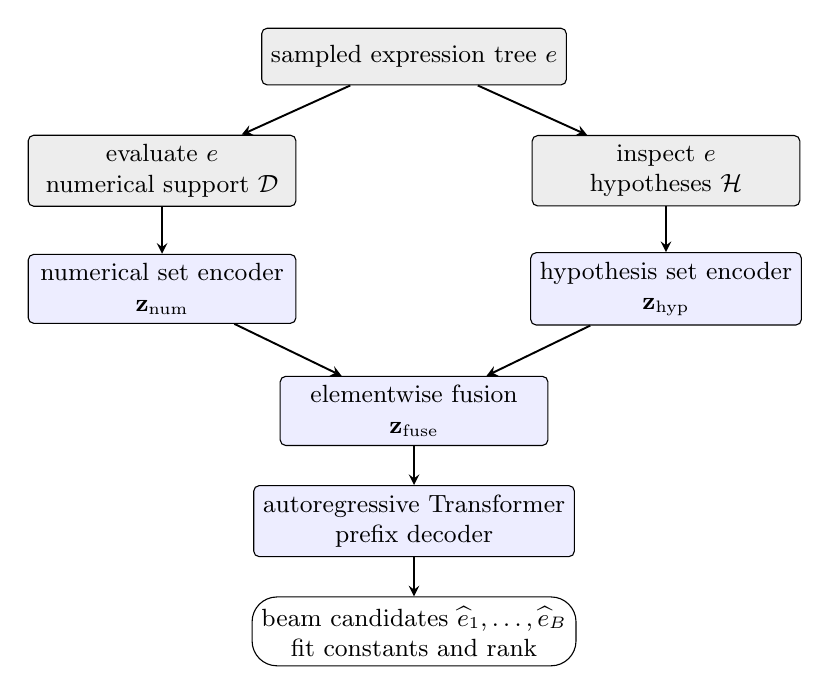
\begin{tikzpicture}[
    block/.style={
        draw,
        rounded corners=2pt,
        fill=blue!7,
        minimum width=3.4cm,
        minimum height=0.72cm,
        align=center,
        font=\small
    },
    source/.style={
        draw,
        rounded corners=2pt,
        fill=black!7,
        minimum width=3.4cm,
        minimum height=0.72cm,
        align=center,
        font=\small
    },
    output/.style={
        draw,
        rounded corners=9pt,
        fill=white,
        minimum width=4.0cm,
        minimum height=0.68cm,
        align=center,
        font=\small
    },
    flow/.style={->,>=stealth,draw,line width=0.7pt}
]
    \node[source] (tree) at (0,3.2)
        {sampled expression tree $e$};
    \node[source] (data) at (-3.2,1.75)
        {evaluate $e$\\numerical support $\mathcal D$};
    \node[source] (hyp) at (3.2,1.75)
        {inspect $e$\\hypotheses $\mathcal H$};
    \node[block] (numenc) at (-3.2,0.25)
        {numerical set encoder\\$\mathbf z_{\mathrm{num}}$};
    \node[block] (hypenc) at (3.2,0.25)
        {hypothesis set encoder\\$\mathbf z_{\mathrm{hyp}}$};
    \node[block] (fuse) at (0,-1.3)
        {elementwise fusion\\$\mathbf z_{\mathrm{fuse}}$};
    \node[block] (decoder) at (0,-2.7)
        {autoregressive Transformer\\prefix decoder};
    \node[output] (candidates) at (0,-4.1)
        {beam candidates $\widehat e_1,\ldots,\widehat e_B$\\
         fit constants and rank};

    \draw[flow] (tree) -- (data);
    \draw[flow] (tree) -- (hyp);
    \draw[flow] (data) -- (numenc);
    \draw[flow] (hyp) -- (hypenc);
    \draw[flow] (numenc) -- (fuse);
    \draw[flow] (hypenc) -- (fuse);
    \draw[flow] (fuse) -- (decoder);
    \draw[flow] (decoder) -- (candidates);
\end{tikzpicture}
\caption{NSRwH training pipeline. The same sampled tree supplies the numerical
observations and the structurally correct hypothesis tokens. At inference, the
two encoder inputs steer a shared prefix-expression decoder.}
\label{fig:nsrwh-pipeline}
\end{figure}

\paragraph{Contribution to the proposed benchmark.}
NSRwH provides a design for controlled mechanism retrieval. The benchmark can
derive $\mathcal H$ automatically from every retained generator tree, then
evaluate recovery under complete, partial, deliberately missing, or partially
incorrect hypotheses. For time series, positive and negative branches can
encode required or forbidden variable--lag subtrees, complexity can control
mechanism size, known constants can expose selected coefficients, and symmetry
can describe exchangeable source variables. The generator remains responsible
for structural, signed, local-contribution, gradient, and Shapley ground truth;
NSRwH supplies a controlled symbolic model whose recovered tree can be compared
with that ground truth.

